\chapter{Nanopore Signal Analysis}
\label{sec:signal}

\begin{itemize}
	\item basics set with pipeline
	\item need to understand signal, contrast to 2nd gen.
	\item tombo, squiggle-kit?
	\item custom, easy to configure
	\item python for fast prototyping
	\item fast5 format, hdfviewer, BulkVis
\end{itemize}

\section{Normalization}
\label{sec:signal:normalization}

\begin{itemize}
	\item mean/std vs median/MAD (cite tombo)
	\item min-max normalization
	\item polyfit?
	\item smoothing with grayscale morphological operations
\end{itemize}

\section{Segmentation and Alignment}
\label{sec:signal:alignment}



\begin{itemize}
	\item estimated event alignment
	\item seqan vs. edlib
	\item event length
	\item profile HMM for precise mapping
\end{itemize}

\begin{figure}[h]
	\centering
	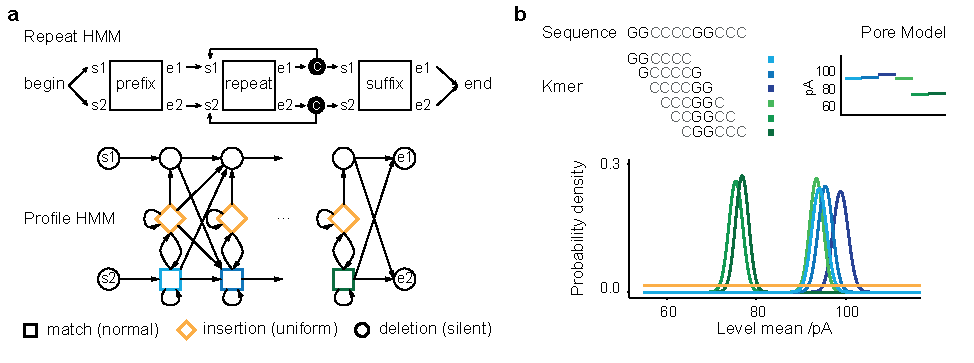
\includegraphics[width=1.0\textwidth]{figures/strique/count_hmm.pdf}
	\captionsetup{format=plain}
	\caption[Nanopore signal processing with STRique]{\textbf{a}, A compound profile HMM of prefix, a single repeat and the suffix sequence assigns either prefix, repeat or suffix label to each signal value. Repeat counts are obtained through dummy states between repeat and suffix. \textbf{b}, Nanopore signal profile HMM with normal distributed match state and uniform distributed insertion state emission probabilities.}
	\label{fig:strique:count_hmm}
\end{figure}